\documentclass{article}
\usepackage{graphicx}
\graphicspath{ {images/} }


\newcommand{\tab}[1]{\hspace{.1\textwidth}\rlap{#1}}

\begin{document}
	
\begin{titlepage}
	\newcommand{\HRule}{\rule{\linewidth}{0.5mm}} % Defines a new command for the horizontal lines, change thickness here

	\center % Center everything on the page
	 
	%----------------------------------------------------------------------------------------
	%	LOGO SECTIONS
	%----------------------------------------------------------------------------------------

	\includegraphics[width=\textwidth]{front-page}

	%----------------------------------------------------------------------------------------
	%	TITLE SECTION
	%----------------------------------------------------------------------------------------

	\HRule \\[0.4cm]
	{ \huge \bfseries Software Requirements Specification}\\[0.4cm] % Title of your document
	\HRule \\[1.5cm]
	 
	%----------------------------------------------------------------------------------------
	%	MEMBERS, TEAM NAME SECTION
	%----------------------------------------------------------------------------------------

	\begin{minipage}{0.5\textwidth}
	\begin{flushleft} \large
	\emph{Members:}\\% add your name and student here
	Peter Boxall 14056136	
	
	Orisha Orrie 13025199
	
	Nsovo Baloyi 12163262
	
	Elizabeth Bode 14310156
		
	Robert Trankle 15092454

	Nikki Constancon 15011713

	Ernst Eksteen 28398603
	\end{flushleft}
	\end{minipage}
	~
	\begin{minipage}{0.4\textwidth}
	\begin{flushright} \large
	{ \huge \bfseries Team Fuchsia }% Title of document
	{\large \today}\\
	{\large v0.1}
	\end{flushright}
	\end{minipage}\\[4cm]
\end{titlepage}


	\newpage
	
	\section{Introduction}
    	
        \subsection{Purpose}
        	\paragraph{The purpose of this document is to put forth a description detailing the NavUP system. It will explain the main purpose of the system, as well as additional subsystems, the interface of these systems, and what they will and will not do, as well as the constraints. Providing a detailed requirement specification of the system as a whole. It is intended for the Client, as well as developers who will integrate the system.}
    	\subsection{Scope}
        	\paragraph{NavUP will be a mobile device application, that will provide the basic functionalities of a navigation system. The system will only interoperate and function on the Hatfield main campus of the University of Pretoria.NavUp will provide a means to navigate the main campus of the University of Pretoria. It will thus provide users choices with regards to which routes they wish to take to reach there destination, taking into account factors such as pedestrian and vehicle traffic as well as providing routes that cater to users who may suffer physical disabilities.NavUP's goal is to provide a personalised, efficient and convenient means of traversing the university's Hatfield campus. The system will also provide extra additional information regarding useful points of interests such as bathroom locations, as well as provide information to the user regarding the rich history of the University of Pretoria.The navigation system will be required to constantly be connected the the campus's WI-FI and will continually send up and down stream information to a server with regards to users location and destination. The server will be required to calculate the route and factor in additional information as set up by the user and there needs. The server must also be able to handle a high volume of concurrent users and provide them all with there required data.Location tracking will be achieved through the use of --WI-FI signal strength and other : not sure of exact methodology-- techniques and not through the use of GPS. /* This means that the two way communication between the device and the server must --explain requirements here-- */ }
        \subsection{Definitions, Acronyms, and Abbreviations}
        \subsection{References}
        \subsection{Overview}
	
	\section{Overall Description}
		
        \subsection{Product Perspective}
        
        	\subsubsection{System Interface}
            \subsubsection{User Interface}            
            \subsubsection{Hardware Interface}
            \subsubsection{Software Interface}
            \subsubsection{Communications Interface}
            \subsubsection{Memory}
            \subsubsection{Operations}
            \subsubsection{Sit Adaption Requirements}
        
		\subsection{Product Functions}
    	\subsection{User Characteristics}    
    	\subsection{Constraints}   
    	\subsection{Assumptions and Dependencies}

	\section{Specific Requirements}
    
    	\subsection{External Interface Requirements}
    	\subsection{Functional Requirements}
    	\paragraph{
Main:
-System shall direct user from current location to desired location.
-System shall inform user on Building informatiom
-The system shall point out high population areas
-The system shall allow user to search for various points of interest
-The System shall show the user various routes to the current destination
-The system shall allow the user to customize the input to create a unique route.

Admin :
-The system shall allow the administrator to Create/Update/delete users.
-The system shall allow the administrator to create/update/delete locations.
-The system shall allow the administrator to create/Update/delete notifications, based on events that occur at UP.
-The system shall generate a report
}

    	Most of the use cases follow all the same functional requirements specification. Figure 1 shows a high-level overview of the system. \\
    	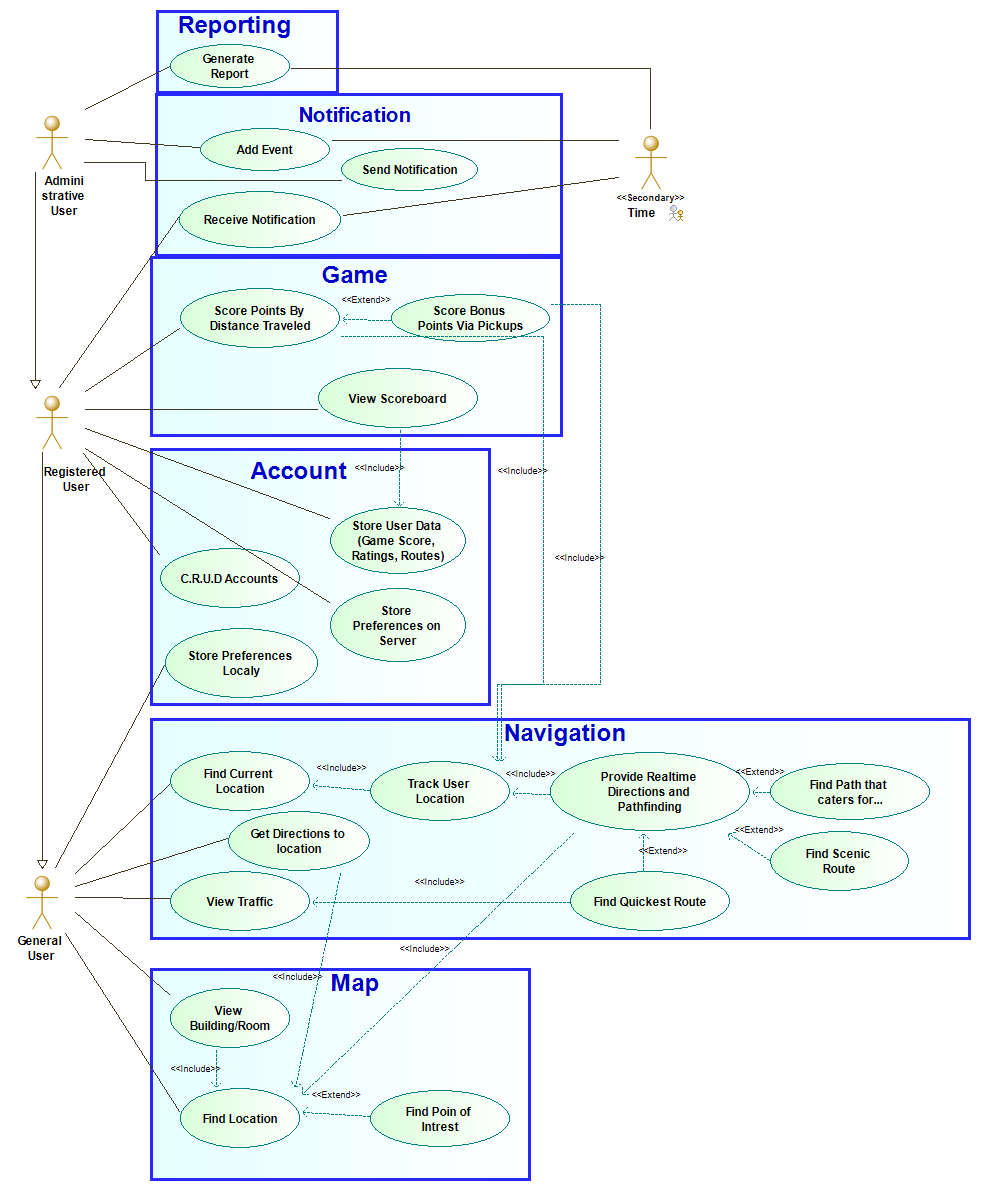
\includegraphics[width=\textwidth]{System_Use_Case_Diagram}
    	
    	\subsubsection{Navigation}
    	The \textit{Navigation} module is responsible for navigation the user from their current location to their desired location.  \\
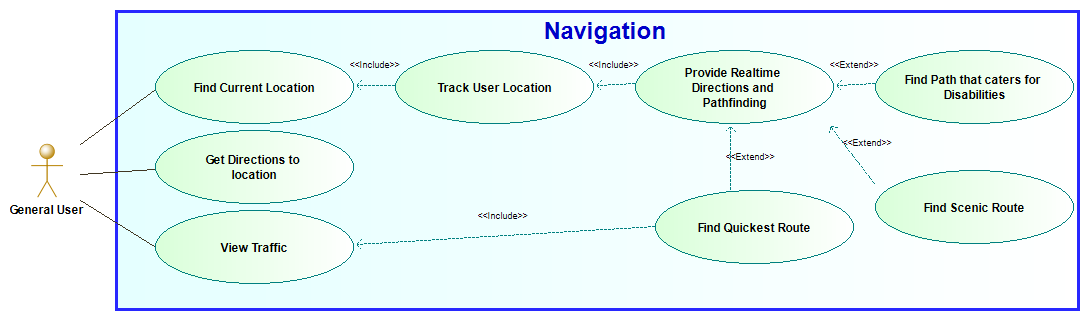
\includegraphics[width=\textwidth]{Navigation_Use_Case_Diagram}
    	\subsubsection{Map}
    	{
	The map system will contain all the stationary information regarding the system, thus it contains the digital information that maps to the real world. A use case exists wherein the general user will be able to search for locations on campus. This use case will be extended to provide functionality whereby the general user can search for specific points of interest on campus, such as toilets and coffee shops. The map system will also allow general users to view buildings and rooms as well as their related information such as historical facts. The map system will also provide the administrative user the rights to C.R.U.D. locations and information regarding those locations.
}
    	\subsubsection{Account}
    	The \textit{Account} module is responsible for management of users using the system. The scope for the \textit{Account} module is shown in Figure 2.  \\[1cm]

\begin{figure}[h]
	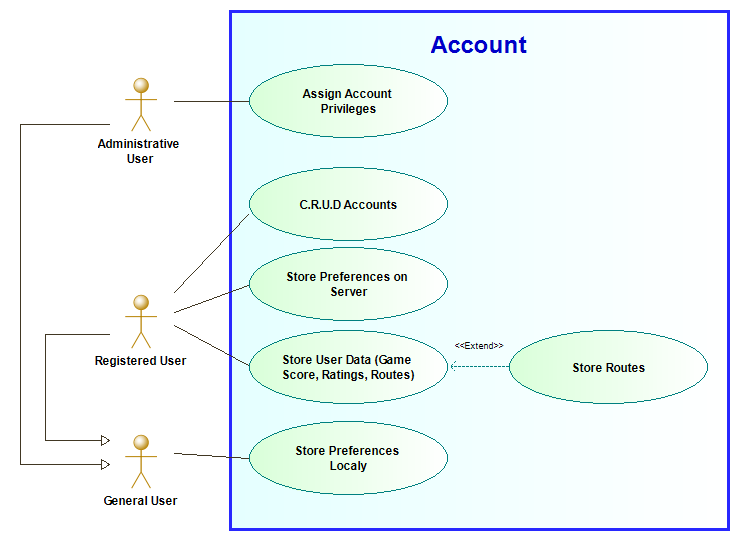
\includegraphics[width=\textwidth]{Account_Use_Case_Diagram}
	\caption{Account module use case}
\end{figure}

\begin{enumerate}
	\item \textbf{Assign Account Privileges}
	\begin{itemize}
		\item Description: \\
		This use case allows the admin user to assign privileges to registered users. He/She may promote or demote users to higher privileges 
		\item Pre-Conditions: \\
		\begin{itemize}
		\item User must be logged in
		\item User must have admin privileges
		\item The admin user must supply a registered user in the request
		
		\end{itemize}
		\item Post-Conditions: \\
		
		\begin{itemize}
		\item The supplied user will have new access privileges 
		
		\end{itemize}
	
	\end{itemize}
	
	\item \textbf{C.R.U.D. Accounts}
	\begin{itemize}
		\item Description: \\
		This use case allow a user to create, update and deactivate an account for the NavUP system
		\item Pre-Conditions: \\
		
		\item Post-Conditions: \\
	
	\end{itemize}
	
	\item \textbf{Store Preferences on Server}
	\begin{itemize}
		\item Description: \\
		
		\item Pre-Conditions: \\
		
		\item Post-Conditions: \\
	
	\end{itemize}
	
	\item \textbf{Store User Data}
	\begin{itemize}
		\item Description: \\
		
		\item Pre-Conditions: \\
		
		\item Post-Conditions: \\
	
	\end{itemize}
	
	\item \textbf{Store Preferences Locally}
	\begin{itemize}
		\item Description: \\
	
		\item Pre-Conditions: \\
		
		\item Post-Conditions: \\
	
	\end{itemize}
\end{enumerate}

    	\subsubsection{Game}
    	The \textit{Game} module is responsible for gamification part of the system. Registered user will be able to collect points and compete with other registered users. The scope of the \textit{Game} module is shown in Figure 5.  \\[1cm]

\begin{figure}[h]
	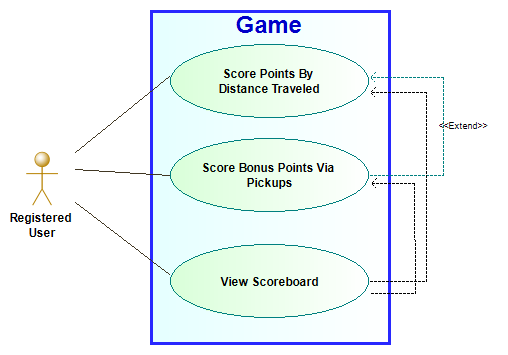
\includegraphics[width=\textwidth]{Game_Use_Case_Diagram}
	\caption{Game module use case}
\end{figure}

\begin{enumerate}
	\item \textbf{Score Points by Distance Travelled}
	\begin{itemize}
		\item Description: \\
		Allows users to score points based on their distance travelled.
		\item Pre-Conditions: \\
		\begin{itemize}
		\item User must be logged in
		
		\end{itemize}
		
		\item Post-Conditions: \\
	
	\end{itemize}
	
	\item \textbf{Score Bonus Points via Pick-ups}
	\begin{itemize}
		\item Description: \\
		Allows users to score points bases on the route travelled
		\item Pre-Conditions: \\
		\begin{itemize}
		\item User must be logged in
		
		\end{itemize}
		
		\item Post-Conditions: \\
	
	\end{itemize}
	
	\item \textbf{View Scoreboard}
	\begin{itemize}
		\item Description: \\
		Allows the user to view their scores
		\item Pre-Conditions: \\
		\begin{itemize}
		\item User must be logged in		
		\end{itemize}
		\item Post-Conditions: \\
	
	\end{itemize}
	
	
\end{enumerate}
    	\subsubsection{Reporting}
    	The \textit{reporting} module is responsible generating and gathering statistical data that can be used for maintenance and system improvement by the administrative team.\\

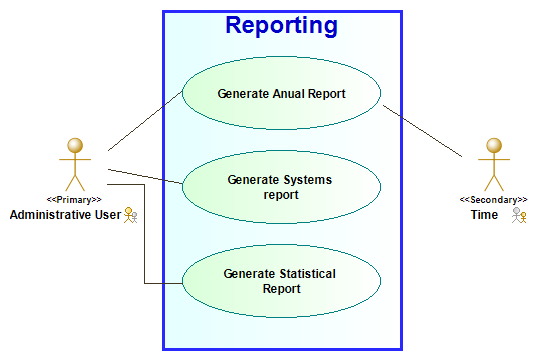
\includegraphics[width=\textwidth]{images/Reporting_Use_Case_Diagram.png}
\begin{center}
	Figure 11: Reporting Module Use Case
\end{center}
    	\subsubsection{Notification}
    	The \textit{notification} module is responsible for managing notifications that are sent from the system to the general user and from the administrative user to general users for items such as events.\\

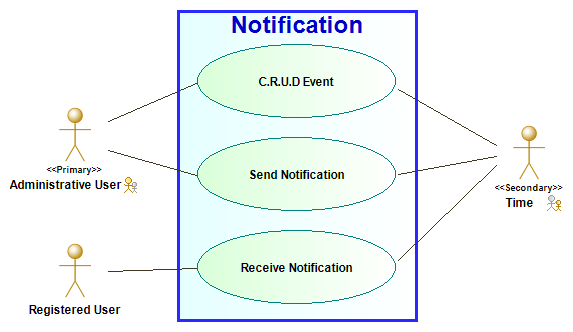
\includegraphics[width=\textwidth]{images/Notification_Use_Case_Diagram.png}

\begin{center}
	Figure 12: Notification Module Use Case
\end{center}
{
The \textit{Notification} system will allow the administrator users to send notifications through to the registered users of the system.
The registered users will then be able to view the notification within the mobile application.
The administrative users will be able to C.R.U.D. events on a day to day basis.
}

        	
        \subsection{Performance Requirements}
        \subsection{Design Constraints}
        \subsection{Software System Attributes}
        \subsection{Other Requirements}
	\begin{itemize}
  		\item The System shall save routes created by the user.
		\item The system shall save the distance traveled, and score it for game purposes.
		\item The system shall save the distances into a leader-board database
		\item The system shall send notifications to the users based on events which occur.
		\item The system shall allow the user to store data (Preferences etc.)
		\item The system shall allow the user to rate routes/parking/points of interestt
	\end{itemize}
	\section{Vision}


	\section{Background}
	
\end{document}
